
%%%%%%%%%%%%%%%%% Introduction to the Assignment %%%

In this Assignment, \textit{\textbf{Problem 3 - Propagation Effects \& Targets}}, ...


%%%%%%%%%%%%%%%%% TASK 1 %%%
\section{Radar Performance}

\subsection{Phenomena affecting radar performance}
The performance of a radar is affected by couple of different phenomena, which degrade or attenuate the sent and received signal.
\begin{enumerate}
	\item \textbf{Atmospheric attenuation} \newline
			Atmospheric attenuation is a major loss term, since the radar beam is attenuated as it's travelling through the atmosphere and its constituents (2-way-loss).
			Water vapor, e.g. clouds, rain or fog, and its density as well as temperature are playing a major role in attenuating the signal. This attenuation is also frequency dependant, e.g. higher frequencies are more attenuated, c.f. fig \ref{fig:attenuation}.
			\begin{figure}[!htbp]
			\centering
			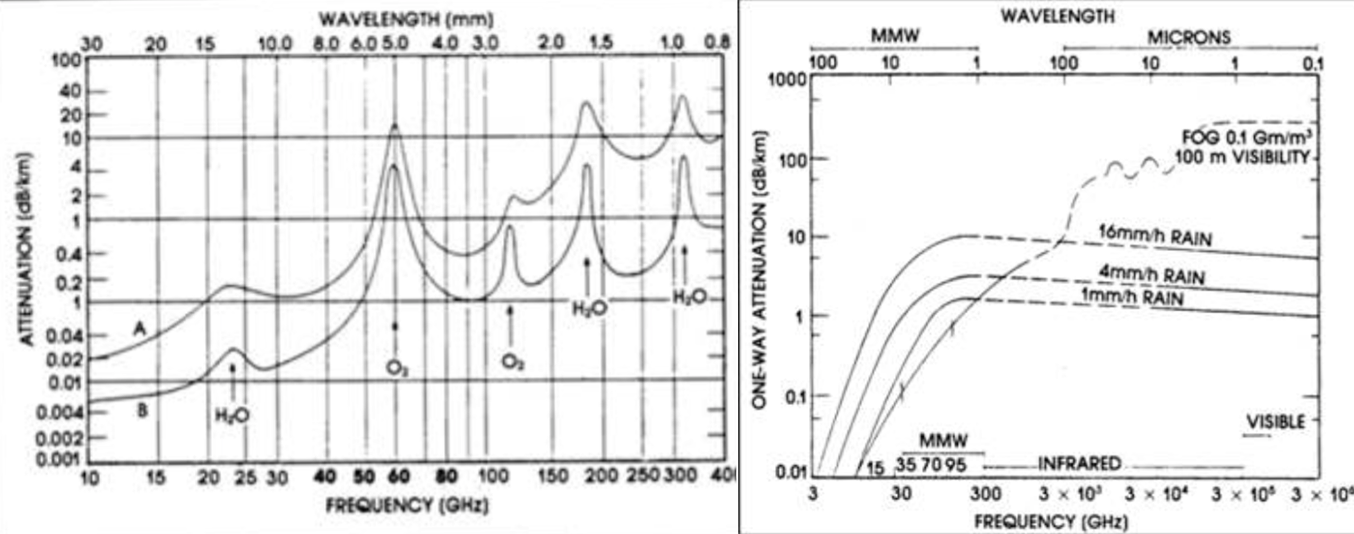
\includegraphics[width=0.9\textwidth]{images/attenuation}
			\caption{atmospheric attenuation as function of frequency \citep{erickson:lecture}}
			\label{fig:attenuation}
			\end{figure}
	\item \textbf{Surface reflection} \newline
			Surface reflection, the reflection of an EM-wave off earth's surface, can lead to multi-path effects when the receiver is hit by the reflected EM-wave, thus leading to measurements that do not correspond with the direction of the original radar beam (assuming an atmospheric radar).
	\item \textbf{Diffraction} \newline
			Diffraction describes the process, when an EM-wave hits an obstacle and is bend around its corners, thus the EM-wave can illuminate things even in a so-called \textit{"shadow zone"}, the zone behind an obstacle. In radar terms, this particular effect can be used to extend the range even beyond the horizon for lower frequencies, since for higher frequencies the diffraction is not very effective.
	\item \textbf{Refraction} \newline
			Atmospheric Refraction is the "bending" of an EM-wave as it propagates through the atmosphere. Refraction is dependant on the constituent of the penetrated material, but also on the thickness of the material and the wavelength of the beam, since the refractive index changes with frequency (optical dispersion) \citep{erickson:lecture}.
	
\end{enumerate}



\subsection{22 GHz and 60 GHz Operation}
Radar is seldom used at 22GHz or 60GHz since at these frequencies the atmosphere is vastly attenuating the signal. Components responsible for the absorption in case of 22GHz is Oxygen ($O_2$) and at 60GHz water vapour ($H_2O$), c.f. fig. \ref{fig:absorb}.
\begin{figure}[h!]
	\centering
	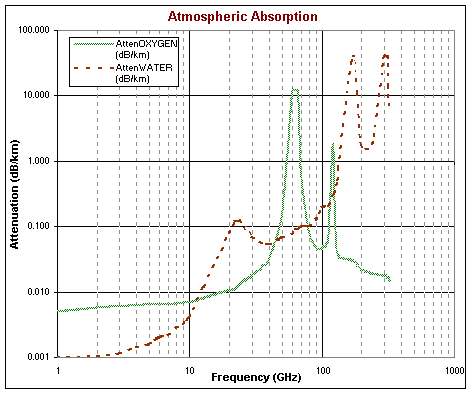
\includegraphics[width=0.7\linewidth]{images/absorbtion}
	\caption{Atmospheric attenuation of different frequencies \protect\footnotemark}	
	\label{fig:absorb}
\end{figure}
\footnotetext{source: \href{http://www.rfcafe.com/references/electrical/images/atm_absorption.gif}{RFCafe}}



%%%%%%%%%%%%%%%%% TASK 2 %%%
\section{Radar cross section (RCS)}

\subsection{Behaviour of normalized RCS}

\subsection{Low specular RCS}


%%%%%%%%%%%%%%%%% TASK 3 %%%
\section{Radar parameters affecting performance}

\subsection{Surface clutter}

\begin{itemize}
	\item \textbf{Pulse width}\newline
		
	\item \textbf{Antenna gain} \newline
	\item \textbf{Transmitter power}\newline
	\item \textbf{Number of pulses returned from target}\newline
	\item \textbf{System losses}\newline
	\item \textbf{Sensitivity of max detection range}
\end{itemize}


\subsection{Receiver noise}


(1) pulse width, (b) antenna gain, (c) transmitter power, (d) number of pulses returned from the target, (e) system losses, and (f) sensitivity of the maximum detection range to changes in the radar cross section.

%%%%%%%%%%%%%%%%% TASK 4 %%%
\section{Atmospheric studies with MF \& HF radars}
Reid (2015) \citep{reid2015mf} reviews different MF and HF partial reflection radar techniques and recent developments, and focuses on the investigation of the neutral upper atmosphere using the aforementioned techniques.


\subsection{Coherent Echoes at 50-110km}
According to Reid, the two main mechanisms that are responsible for the coherent echoes from the MLT\footnote{Mesosphere and Lower Thermosphere} region are Bragg, or turbulent, Scatter and Fresnel Scatter. \\
Bragg Scatter is the return of radar waves due to turbulent irregularities in the electron density of the observed volume. \\
Fresnel Scatter is the partial reflection that is the result of irregularities in the refractive index orthogonal to the radar beam direction, where the irregularities are very thin compared to the wavelength of the radar beam \citep{reid2015mf}.

\subsection{Choice of operational frequency \& optimal PRF}

The operational frequency of a radar used for atmospheric studies is usually determined by the available spectrum and licensing, where the chosen frequency is mostly a compromise between licensing, preferably lower frequencies for good backscattered power and the reflection height, which prefers higher frequencies \citep{reid2015mf}. Also, the latitude, time of day, season and solar cycles play a role in determining the reflection height \citep{jursa1985handbook}.

The optimal Pulse Repetition Frequency is depending on the total reflection height, meaning the total height, respectively the range, where the atmosphere shall be observed.
\begin{figure}[h]
	\centering
	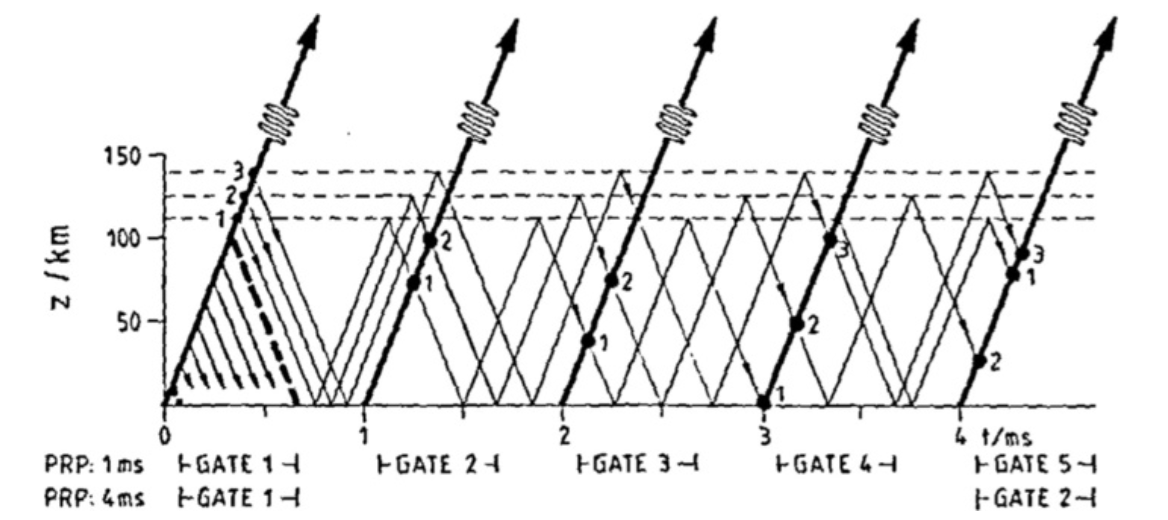
\includegraphics[width=0.8\textwidth]{images/maxPRF}	
	\caption{Range-time diagram \citep[c.f.][Fig. 5]{reid2015mf} }
\end{figure}


\subsection{Main Principle of spaced antenna techniques}
Spaced Antenna (SA) techniques are usually used for investigating and observing ionospheric dynamics and to measure the "apparent motion of ground diffraction pattern across the observing region" \citep{reid2015mf}.\\
In a default operational configuration the transmitting antenna is located close to minimum three non-collinear receiving antennas to receive partial reflections from the D-region. The antennas usually work in a bi-static mode, which means there are separate antennas for transmitting and receiving. But it is also common that the same antennas are used for both transmitting and receiving, e.g. as illustrated in fig. \ref{fig:SAconfing}, where in this particular case each antenna has its own receiver \citep{reid2015mf}.

\begin{figure}
	\centering
	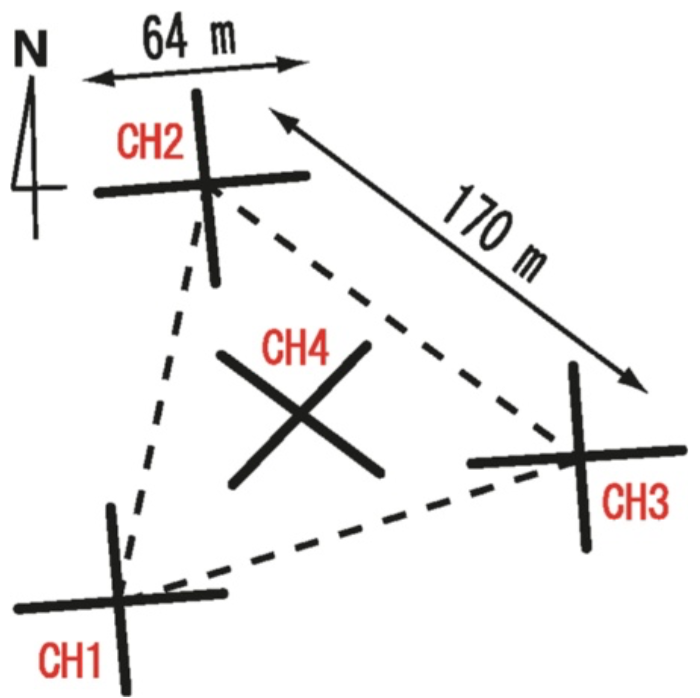
\includegraphics[width=0.5\textwidth]{images/SA_config}
	\caption{typical SA configuration at 2.43MHz (Poker Flat MF radar) \citep[c.f][Fig. 2]{reid2015mf} }
	\label{fig:SAconfing}
\end{figure}

To analyse the received signals at the three receiver antennas usually a simple correlation analysis is exerted to determine the diffraction pattern motion of the partial reflections from the D-region. In the typical case one uses coherent receivers and only the amplitude information for the analysis \citep{reid2015mf}.

One of the advantages of this particular technique is the wide angular polar diagram one obtains when the backscatter angle is wide, thus resulting in a wide effective beam.\\
Still, this technique has some disadvantages, as for example a large area is required to place the antennas. And also the antennas need a large dynamic range for the returned echo power, which is a problem for especially older systems, since those may not have sufficient digitization capabilities \citep{reid2015mf}.

\subsection{Apparent and true velocity}
The apparent velocity is the motion of the ground diffraction pattern over the spaced antenna location, and is calculated using the time delays of the cross-correlation function which is determined between the pairs of antennas. The apparent vertical velocity is measured utilizing the phase of the complex autocorrelation function. \\
Using that simple correlation analysis, basically being a similar fades analysis, one does not take into account random changes in the pattern motion and the anisotropy in the pattern, as the pattern moves. This results in an overestimation of the \textit{true velocity} magnitude. \\
Thus, the true velocity describes the velocity, that takes into account the just stated phenomena, basically a corrected version of the apparent velocity.
\todo{include Fig 12 from REID paper}


\subsection{Deficiency of full correlation analysis for MF/HF}

The major flaw of the Full Correlation Analysis (FCA) is the very high underestimation of wind magnitude of 15\% to 40\% for an ideally configured system. According to Reid \citep{reid2015mf} this is an unacceptably high number for studies of wind dynamics. This bias is highly height dependant for MF and HF SA radars, but the reason for this is not fully understood, though the assumption of insufficient sampling of the ground diffraction pattern has been made \citep{reid2015mf}.






